% !TeX TS-program = pdflatex
% !TeX encoding = UTF-8
% !TeX spellcheck = en_US

\documentclass[a4paper]{article}

%define this conditional; plasTeX will override it and set it to `true`
\newif\ifplastex\plastexfalse

%% fallback for older LaTeX, to use checkpoints
\ifplastex\else
 \ifdefined\CurrentFile\else
 \usepackage{currfile}
 \fi
\fi
%%%%%%%%% early packages that for some reason must be loaded before

%% `unicode-math` will change some definitions in `amssymb`
\usepackage{amssymb}

%% some older versions of `hyperref` clash with `iftex`
\usepackage{hyperref}

%%%%%%%%%% prepare conditionals
% http://ctan.mirror.garr.it/mirrors/CTAN/macros/latex/contrib/iftex/iftex.pdf
% you need a recent version
\usepackage{iftex}

%
%%%%%%%%% use conditionals to load some engine-specific packages
\ifplastex
  % code for plastex
  \newcommand\mathbbm[1]{{\mathbb{#1}}}
\else\iftutex
  % code for xetex or luatex
  \ifluatex
   \usepackage{luatextra}
\fi
\usepackage{polyglossia}
\usepackage{fontspec}
\usepackage[math-style=ISO,bold-style=ISO]{unicode-math}
%% http://tex.stackexchange.com/questions/55204/remapping-latex-symbol-to-another-unicode-value/55205
\AtBeginDocument{\let\setminus\smallsetminus}
\newcommand\mathbbm[1]{{\mathbb{#1}}}

\else
 % code for (pdf)latex
      \usepackage{lmodern}
   \usepackage{amsfonts}
   \usepackage[utf8]{inputenc}
   \usepackage[english,italian]{babel}
   \IfFileExists{bbm.sty}
    {\usepackage{bbm}}
    {\newcommand\mathbbm{\mathbb}}


\ifCDLeng \selectlanguage{english}\fi
\ifCDLita \selectlanguage{italian}\fi

\fi\fi

\usepackage{makeidx}
\makeindex


%%%%%%%%% following are general definitions

\usepackage{amsthm,amsmath}

\usepackage{graphicx}

\usepackage{makeidx}
\makeindex

% use \index for language-agnostic content
% use \indexLita for italian keywords
% use \indexLeng for english keywords
\ifCDLita
 \newcommand\indexLita[1]{\index{#1}}
\else
 \newcommand\indexLita[1]{}
\fi
\ifCDLeng
 \newcommand\indexLeng[1]{\index{#1}}
\else
 \newcommand\indexLeng[1]{}
\fi

\usepackage{lipsum}

\newcounter{myCount}
\newtheorem{Defn}[myCount]
{\ifCDLeng Definition\fi\ifCDLita Definizione\fi}
\newtheorem{Theorem}[myCount]
{\ifCDLeng Theorem\fi\ifCDLita Teorema\fi}
\newtheorem{Cor}[myCount]
{\ifCDLeng Corollary\fi\ifCDLita Corollario\fi}
\newtheorem{Lem}[myCount]{Lemma}

\newenvironment{privateremark}{[}{]}

\newenvironment{buyablecontent}{[}{]}

%% you may customize the appearance of the marker written by the \uuid command
%%
% \renewcommand{\uuidformatter}[1]{{\texttt{[#1]}}}
%%
%% See in ColDocUUID.sty


\ifplastex
%% plastex currently does not know eqref
\def\eqref{\ref}
\fi

% math entities, that may be converted to unicode with ColDoc web interface
\newcommand\reals{{\mathbb{R}}}
\newcommand\integers{{\mathbb{Z}}}



\begin{document}
\author{J. Smith
\emph{et al}
}
\title{That papert}
\maketitle
\section*{Introduction}
The introduction

\begin{abstract}
  This simple \LaTeX\ tests some features
  of \texttt{plasTeX} and \texttt{ColDoc}.

  \ifetex Using  \TeX \fi ;
  \ifxetex Using \texttt{XeTeX} \fi ;
  \ifluatex Using \texttt{LuaTeX} \fi ;
  \iftutex Using \texttt{XeTeX} or \texttt{LuaTeX} \fi ;
  \ifplastex Using \texttt{plasTeX} \fi .

  %% this works only inside the portal
  %\ifColDocPublic Public \else Private \fi version, compiled
  %\ifColDocOneUUID only this UUID \else as a whole \fi.
\end{abstract}

Stress test  \texttt{plasTeX} embedding \texttt{HTML}
\begin{verbatim}
<a href="http://www.debian.org">Debian</a>
\end{verbatim}
\[ \hbox{<a href="http://www.debian.org">Debian</a>} \]

BBM test for bold ``1''
\[f={\mathbbm{1}}_A\]
\index{BBM test}

\begin{buyablecontent}
  This content is reserved but it may be bought
\end{buyablecontent}

\begin{privateremark}
  This is a private remark that only the author will see
\end{privateremark}

\section{\ifCDLeng Content\fi \ifCDLita Contenuto\fi}

\subsection{\ifCDLeng Notation\fi \ifCDLita Notazioni\fi}

\begin{Defn}
  \label{defn:1}
  \CDLeng Some definitions, $\cos(x)$ and \(\sin(x)\) are
  \CDLita Alcune definizioni $\cos(x)$ e \(\sin(x)\) sono
  \begin{eqnarray}
    \CDLeng \tan \label{english_only}\\
    \cos(x) \doteq \frac{e^{ix}+e^{-ix}}{2}  \label{eq:fefwe} \\
    \sin(x) \doteq \frac{e^{ix}-e^{-ix}}{2i} \label{eq:fefwe2}
  \end{eqnarray}
  \CDLeng A reference to a figure \ref{fig:a354}.
  \CDLita Un riferimento alla figura   \ref{fig:a354}.
  %
  \CDLeng A reference \eqref{eq:fefwe} and  \eqref{eq:fefwe2} to the above equations.
  \CDLita Un riferimento a \eqref{eq:fefwe} e  \eqref{eq:fefwe2} nelle equazioni precedenti.
\end{Defn}

\CDLeng A reference \eqref{english_only},\eqref{eq:fefwe} and  \eqref{eq:fefwe2} to the above equations.
\CDLita Un riferimento a \eqref{eq:fefwe} e  \eqref{eq:fefwe2} nelle equazioni precedenti.


\begin{figure}[ht]\label{fig:a354}
  \begin{center}
    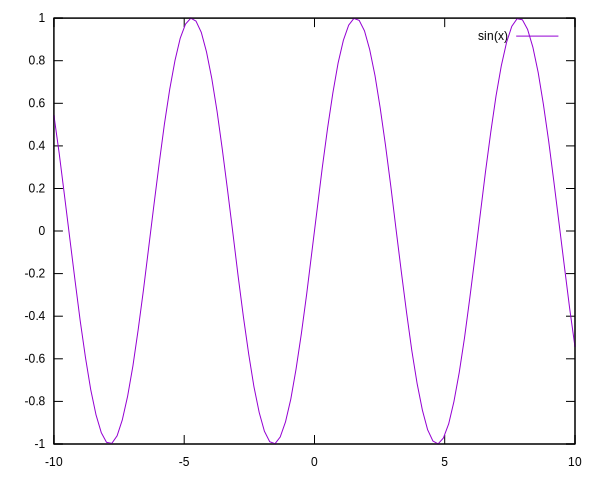
\includegraphics[width=0.5\textwidth]{F/sin}
    \caption{Graph of \(\sin(x)\).}
  \end{center}
\end{figure}




%%% Local Variables:
%%% mode: latex
%%% TeX-master: "paper"
%%% TeX-engine: xetex
%%% End:


\subsection{Proofs}

\begin{Lem}[A Lemma]\label{lem:1}
  \lipsum[3]
\end{Lem}

\begin{Theorem}[The main theorem]\label{thm:1}
  Using Definition \ref{defn:1} \\
  \lipsum[4]
  \begin{proof}
    using Lemma \ref{lem:1} and
    \begin{equation}
      \label{eq:1}
      {\mathbf{e}}^{i \pi }=-1
    \end{equation}
  \end{proof}
  This tests \texttt{MathJax}: $x<y$ or $x>y$
\end{Theorem}

\lipsum[5]

\begin{Cor}\label{cor:1}
  Corollary to Theorem \ref{thm:1}.
  \\
  \lipsum[6]
\end{Cor}

%%% Local Variables:
%%% mode: latex
%%% TeX-master: "paper"
%%% End:


\begin{description}
  % a nasty comment
\item[one] 1
\item[two] 2 %due
\item[three] 3
\end{description}

\section*{Table of contents}
\tableofcontents

\printindex

\bibliographystyle{plain}
\bibliography{subdir/paper}

\begin{thebibliography}{9}
\bibitem{latexcompanion}
Michel Goossens, Frank Mittelbach, and Alexander Samarin. 
\textit{The \LaTeX\ Companion}. 
Addison-Wesley, Reading, Massachusetts, 1993.

\bibitem{einstein} 
Albert Einstein. 
\textit{Zur Elektrodynamik bewegter Korper}. (German) 
[\textit{On the electrodynamics of moving bodies}]. 
Annalen der Physik, 322(10):891–921, 1905.

\bibitem{knuthwebsite} 
Knuth: Computers and Typesetting,
\\ \url{http://www-cs-faculty.stanford.edu/~uno/abcde.html}
\end{thebibliography}

\end{document}
  
%%% Local Variables:
%%% mode: latex
%%% TeX-master: t
%%% End:
